% Editable, colorblind-safe PGFPlots source (Okabe--Ito palette).
% Source: unified_quadrature_bias_v1/results/full_development_20seeds.json
% Residual values are reported in prose, deliberately avoiding a dual-axis chart.
% A logarithmic count axis keeps all four nonzero counts visually distinguishable.
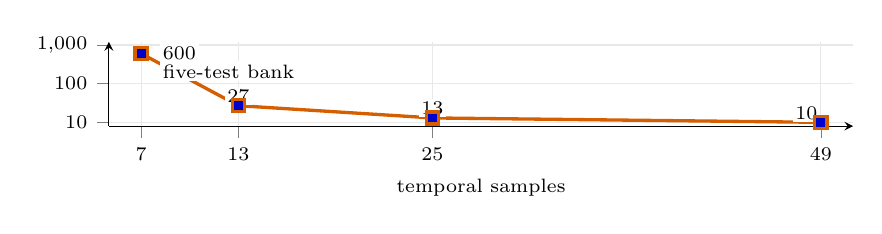
\begin{tikzpicture}
\begin{axis}[
  width=0.91\linewidth,
  height=2.65cm,
  xmin=5,xmax=51,
  ymode=log,
  log basis y=10,
  ymin=8,ymax=1200,
  xtick={7,13,25,49},
  ytick={10,100,1000},
  yticklabels={10,100,{1,000}},
  xlabel={temporal samples},
  ylabel={},
  axis lines=left,
  tick align=outside,
  grid=major,
  grid style={gray!18},
  label style={font=\scriptsize,align=center},
  tick label style={font=\scriptsize},
]
\addplot+[very thick,color={rgb,255:red,213;green,94;blue,0},mark=square*,mark size=2.2pt]
  coordinates {(7,600) (13,27) (25,13) (49,10)};
\node[font=\scriptsize,anchor=west,fill=white,inner sep=1.2pt] at (axis cs:8.1,600) {600};
\node[font=\scriptsize,anchor=south,fill=white,inner sep=1.0pt] at (axis cs:13,27) {27};
\node[font=\scriptsize,anchor=south,fill=white,inner sep=1.0pt] at (axis cs:25,13) {13};
\node[font=\scriptsize,anchor=south east,fill=white,inner sep=1.0pt] at (axis cs:49,10) {10};
\node[font=\scriptsize,anchor=north west,fill=white,inner sep=1.2pt]
  at (axis cs:8.1,390) {five-test bank};
\end{axis}
\end{tikzpicture}
